\documentclass[a4paper,12pt]{report}
\usepackage{latexsym}
\usepackage[MeX]{polski}
\usepackage[utf8]{inputenc}	% kodowanie znaków
\usepackage{listings} 		% kolorowanie składni
\usepackage{color}		% kolory
\usepackage{xcolor}		% bonusowe kolory
\usepackage{hyperref}	% linki w spisie treści, odnośniki, zakładki w pdf
\usepackage{upquote}  	% zamiana cudzysłowów klasycznych (,, ") na górne (" ") w kodach źródłowych
\usepackage{graphicx}	% wskawianie obrazków

% Ustawienie marginesów
\oddsidemargin=0cm
\topmargin=0cm
\textwidth=16cm
\textheight=23cm

% Ustawienie ładnych etykiet do kodów źródłowych
\usepackage{caption}		
\DeclareCaptionFont{white}{\color{white}}
\DeclareCaptionFormat{listing}{\colorbox{gray}{\parbox{\textwidth}{#1#2#3}}}
\captionsetup[lstlisting]{format=listing,labelfont=white,textfont=white}


%Zdefiniowanie autora i~tytułu:
\author{Kacper Szkudlarek, Maciej Stefańczyk}
\title{PUCY MP\_02}

\frenchspacing


%%
%% AHDL definition
%%
\lstdefinelanguage{AHDL}%
  {morekeywords={AND,BEGIN,BIDIR,BITS,BURIED,CARRY,CASCADE,CASE,CLIQUE,CONNECTED_PINS,CONSTANT,
DEFAULTS,DESIGN,DEVICE,DFF,DFFE,ELSE,ELSIF,END,EXP,FUNCTION,GLOBAL,GND,IF,INCLUDE,INPUT,IS,JKFF,JKFFE,
LATCH,LCELL,MACHINE,MACRO,MCELL,NAND,NODE,NOR,NOT,OF,OPTIONS,OR,OTHERS,OUTPUT,RETURNS,SRFF,SRFFE,
SOFT,STATES,SUBDESIGN,TABLE,TFF,TFFE,THEN,TITLE,TRI,VARIABLE,VCC,WHEN,WITH,X,XNOR,XOR},% 
   sensitive=f,
   morecomment=[l]--,%
   morecomment=[s]{\%}{\%},%
   morestring=[d]{"}%
  }[keywords,comments,strings]%

\lstdefinelanguage{oasm}%
  {morekeywords={STOP, RESET, JMP, JZ, ADD, SUB, LD, OR, AND, LDI, IN, OUT, STORE, MUL},%
   sensitive=f,%
   morecomment=[l];,% nonstandard
  }[keywords,comments]%

\lstset{
	language=,	                		% choose the language of the code
	basicstyle=\footnotesize\ttfamily,       	% the size of the fonts that are used for the code
	numbers=left,                   		% where to put the line-numbers
	numberstyle=\tiny,      			% the size of the fonts that are used for the line-numbers
	stepnumber=1,                   		% the step between two line-numbers. If it's 1 each line will be numbered
	numbersep=5pt,                  		% how far the line-numbers are from the code
	showspaces=false,               		% show spaces adding particular underscores
	showstringspaces=false,         	% underline spaces within strings
	showtabs=false,                 		% show tabs within strings adding particular underscores
	tabsize=4,	                		% sets default tabsize
	captionpos=t,                   		% sets the caption-position
	breaklines=true,                		% sets automatic line breaking
	breakatwhitespace=true,        	% sets if automatic breaks should only happen at whitespace
	extendedchars=true,
	keywordstyle=\color{blue}\bfseries,
	commentstyle=\color{gray}\textit,
}

\begin{document}

%Wstawienie autora i~tytułu do składu:
\maketitle

%Wstawienie spisu treści:
\tableofcontents



%%%%%%%%%%%%%%%%%%%%%%%%%%%%%%%%%%%%%%%%%%%%%%%%
% Wiadomości ogólne o całym projekcie
%%%%%%%%%%%%%%%%%%%%%%%%%%%%%%%%%%%%%%%%%%%%%%%%
\chapter{Realizacja ogólna}

\section{Treść zadania}

Tutaj trzeba wstawić treść naszego zadanka ;-)

\section{Założenia projektowe}

Założenia projektowe które przyjeliśmy

\section{Schemat blokowy układu}

Schemat blokowy - w sumie trzeba przerysować to z treści

%%%%%%%%%%%%%%%%%%%%%%%%%%%%%%%%%%%%%%%%%%%%%%%%
% Dokładne opisy poszczególnych komponentów
%%%%%%%%%%%%%%%%%%%%%%%%%%%%%%%%%%%%%%%%%%%%%%%%
\chapter{Opis komponentów}

\section{Moduł CPU}


\section{Pamięć RAM}


\section{Pamięć ROM}


\section{Moduł operacji złożonej -- mnożenie Bootha}

Algorytm Bootha jest wykorzystywany do mnożenia dwóch liczb binarnych zapisanych w postaci U2.

Algorytm polega na sukcesywnym dodawaniu do sumy częściowej P jednej z dwóch predefiniowanych wartości -- A bądź S. Oznaczmy przez m i r mnożną i mnożnik naszego działania, a przez n ich ilość bitów.

\begin{enumerate}
  \item Ustalenie początkowych wartości A, S i P (każde z nich powinno być długości 2n+1 bitów)
  \begin{enumerate}
    \item Wypełnienie najstarszych n bitów liczby A wartością m, pozostałe bity zerujemy (A = \{m, 0..0\})
    \item Wypełnienie najstarszych n bitów liczby S wartością -m (w dopełnieniu do 2), pozostałe bity zerujemy (S = \{-m, 0..0\})
    \item Wypełniamy najstarsze bity P zerami, nastepnie wstawiamy liczbę r, a najmłodszy bit ustawiamy na 0 (P = \{0..0, r, 0\})
  \end{enumerate}
  \item Jeśli dwa najmłodsze bity sumy częściowej P wynoszą:
  \begin{enumerate}
    \item 01 -- P = P + A
    \item 10 -- P = P + S
    \item 00 lub 11 -- P pozostaje bez zmian
  \end{enumerate}
  \item Przesunięcie arytmetyczne P o jeden bit w prawo
  \item Powtórzenie kroków od 2 i 3 w sumie n razy
  \item Wynikiem mnożenia jest P po usunięciu najmłodszego bitu (przesunięciu bitowym w prawo)
\end{enumerate}

W projekcie mnożenie zostało zrealizowane jako osobny blok funkcjonalny, do którego podawane są mnożna i mnożnik. Blok ten posiada własny sygnał WAIT oznaczający trwające obliczenia, a po ich zakończeniu wynik jest udostępniany przy pomocy odpowiednich sygnałów. Obie liczby na wejściu muszą być tej samej długości (w projekcie przyjęto n=8, ale łatwo jest to zmienić), wynik natomiast jest dwukrotnie dłuższy (ze względu na architekturę projektowanego mikrokontrolera odczytywane jest tylko 8 młodszych bitów).

\section{Układ wejścia -- klawiatura PS/2}

\begin{figure}[h]
\centering
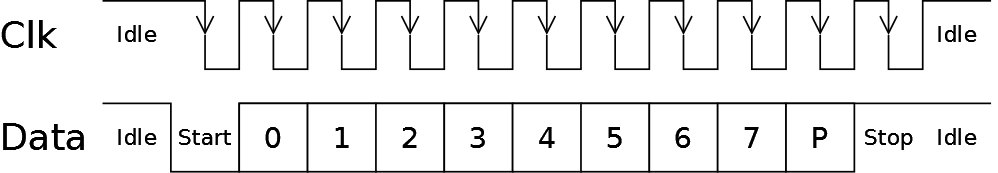
\includegraphics[width=8cm]{./pict/PS2.png}
\caption{Przebiegi czasowe na liniach portu PS/2 podczas transmisji pojedynczego znaku z klawiatury.}
\label{fig:ps2}
\end{figure}

\section{Układ wyjścia -- drukarka LPT}

\begin{figure}[h]
\centering
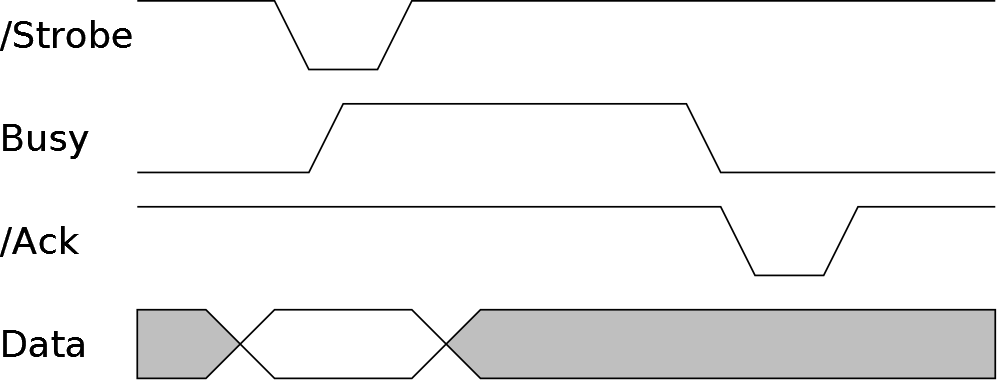
\includegraphics[width=8cm]{./pict/LPT.png}
\caption{Przebiegi czasowe na najważniejszych liniach portu LPT podczas wysyłania danych.}
\label{fig:lpt}
\end{figure}

%%%%%%%%%%%%%%%%%%%%%%%%%%%%%%%%%%%%%%%%%%%%%%%%
% Opis assemblera
%%%%%%%%%%%%%%%%%%%%%%%%%%%%%%%%%%%%%%%%%%%%%%%%
\chapter{Assembler}

\section{Opis}

W celu ułatwienia testowania układu stworzony został prosty program mający na celu tłumaczenie kodu programu z postaci źródeł assemblera na pliki .mif wczytywane przez program Quartus. Program, pomimo swojej prostoty, w znaczący sposób skrócił czas tworzenia programów testowych, a także wyeliminował potencjalne błędy mogące powstać podczas ręcznego uzupełniania zawartości ROMu.

Prostota programu nie oznacza jednak, że jest on bardzo ograniczony. Wręcz przeciwnie -- został napisany w sposób umożliwiający bardzo łatwe zaadaptowanie go do różnych architektur i zestawów instrukcji. Poprzez modyfikację pliku z definicją języka można zmienić długość kodów operacji, dodać nowe instrukcje, modyfikować ilość rejestrów wewnętrznych procesora, tworzyć nowe typy instrukcji (różne ilości i typy operandów).

\section{Instrukcja użycia}

\subsection{Definicja języka}

Plik z definicją języka podzielony jest na 3 sekcje:
\begin{itemize}
  \item definicja instrukcji
  \item definicja rejestrów
  \item definicja typów instrukcji
\end{itemize}

Każdy z sektorów musi zaczynać się liczbą oznaczającą ilość jego wpisów, a cały plik nie powinien zawierać pustych linii. Każdy wpis powinien być umieszczony dokładnie w jednej linii.

\subsubsection{Definiowanie instrukcji}
Ogólna postać definicji pojedynczej instrukcji składa się z 3 części:
\begin{itemize}
  \item Kod operacji w postaci binarnej -- wstawiany jest bezpośrednio w pliku wynikowym. Jego długość nie jest okreslona, ale dla danego typu instrukcji powinna być stała (każda instrukcja powinna w sumie składać się z pełnych bajtów).
  \item Mnemonik instrukcji -- tekstowy odpowiednik instrukcji używany w kodach źródłowych, podczas parsowania zastępowany odpowiednim kodem.
  \item Typ instrukcji -- jeden z typów określonych w 3 sekcji pliku z definicją języka. Określa ilość i typy parametrów dla danej instrukcji.
\end{itemize}

\subsubsection{Rejestry procesora}

W drugiej sekcji zawarta jest prosta definicja rejestrów dostepnych dla danej architektury. Każda linia składa się z nazwy symbolicznej rejestru i następujągo po niej binarnego kodu daneg rejestru (który wykorzystywany jest podczas tworzenia pliku wynikowego jako część instrukcji).

\subsubsection{Definiowanie typów instrukcji}

Trzecia sekcja pliku z definicją języka zawiera zdefiniowane typy instrukcji (do nich własnie odnoszą się typy z sekcji pierwszej). Każdy typ składa się z 2 głównych części: liczbiwego kodu typu oraz definicji składni instrukcji danego typu.

Definicja składni może zawierać jeden bądź wiele elementów składowych, z których kazdy oznacza, jak wynikowo powinna zostać złozona instrukcja, a także jakiego typu parametry są dozwolone. Możliwe wartości do wstawienia w tym miejscu to:
\begin{itemize}
  \item OPCODE -- kod instrukcji (mnemonik w kodzie źródłowym, binarny kod operacji w pliku wynikowym)
  \item Rd -- symboliczna nazwa jednego z rejestrów, zamieniana na jego kod w pliku wynikowym
  \item IM8 -- liczba całkowita (w postaci dziesiętnej bądź szesnastkowej poprzedzonej '0x'), w pliku wynikowym zapisywana w postaci 8-bitowej
  \item IM16 -- jak IM8, tyle że w pliku wynikowym zamieniana na liczbę 16-bitową
  \item 0 -- w tym miejscu w pliku wynikowym zostanie wstawione jedno 0, nie wpływa na postać instrukcji w kodzie źródłowym. Używane do wyrównywania instrukcji do wielokrotności 8 bitów.
\end{itemize}

\subsection{Pliki źródłowe}

Format plików źródłowych jest dość prosty, podobny do standardowych plików assemblera. Instrukcje zapisywane są przy pomocy kodów określonych w definicji języka, argumenty oddzielone mogą być przecinkiem, spacją, tabulatorem bądź dowolną ich kombinacją. 

Komentarze dostępne są jedynie w wersji całej linii (linia komentarza powinna zaczynać się od średnika). Wszystkie komentarze umieszczone na początku pliku przed pierwszą linią z kodem bądź przed pierwszą pustą linią są umieszczane na początku pliku wynikowego, pozostałe komentarze umieszczane są w pliku wynikowym bezpośrednio przed kodem wygenerowanym z następnej instrukcji.

\subsection{Kompilacja}

\section{Przykłady}

\subsubsection{Assembler dla procesora z projektu}
\lstset{
tabsize=6
}
\begin{lstlisting}[caption=Definicja języka,language=]
14
00000	STOP	0
00001	RESET	0
00010	JMP	1
00011	JZ	2
00100	ADD	3
00101	SUB	3
00110	LD	3
01000	OR	3
01001	AND	3
01010	LDI	2
01011	IN	2
01100	OUT	2
01110	STORE	4
10100	MUL	3
8
R0	000
R1	001
R2	010
R3	011
R4	100
R5	101
R6	110
R7	111
5
0	OPCODE 0 0 0
1	OPCODE 0 0 0 IM8
2	OPCODE Rd IM8
3	OPCODE Rd 0 Rd 0 Rd
4	OPCODE Rd IM16
\end{lstlisting}

Dostępnych jest 14 instrukcji 5 typów, każda z nich ma 5-bitowy kod. Procesor wyposażony jest w 8 rejestrów, każdy z nich o 3-bitowym kodzie. Typy instrukcji można przetłumaczyć następująco:
\begin{itemize}
  \item 0 -- instrukcja składa się jedynie z samego kodu operacji, pozostałe zera służą do dopełnienia długości kodu wynikowego do wielokrotności 8 bitów. Instrukcja bezargumentowa.

  Przykład: STOP -- zatrzymanie wykonywania programu
  \item 1 -- Instrukcja posiadająca jeden argument typu całkowitoliczbowego, 8 bitowego. 

  Przykład: JMP 0x20 -- skok bezwarunkowy pod podany adres
  \item 2 -- instrukcja posiadająca dwa argumenty -- w kolejności symbol rejestru oraz stałą liczbową 8-bitową.
  
  Przykład: LDI R3, -123 -- załadowanie do rejestru R3 wartości -123
  \item 3 -- instrukcja posiadająca 3 argumenty, wszystkie będące symbolami rejestrów.

  Przykład: ADD R2, R3, R4 -- dodanie rejestrów R3 i R4, umieszczenie wyniku w rejestrze R2
  \item 4 -- instrukcja posiadająca dwa argumenty - symbol rejestru oraz stała liczbową 16-bitową.

  Przykład: STORE R5, 0x1234 -- zapisanie wartości rejestru R5 do pamięci RAM pod adres 0x1234.
\end{itemize}


\lstset{
tabsize=6,
morekeywords={IN, ADD, OUT, MUL}
}
\begin{lstlisting}[caption=Przykładowy kod programu,label=asm_1,language=oasm]
; Simple test program for VHDL general-purpose CPU
; Authors:
; 	Maciej Stefanczyk
;	Kacper Szkudlarek

	IN	R0, -1
	IN	R1, -1
	ADD	R2, R1, R0
	OUT	R2, 0
	IN	R1, -1
	MUL	R3, R1, R2
	OUT	R3, 0

; stop operation
	STOP
\end{lstlisting}

\lstset{
tabsize=6
}
\begin{lstlisting}[caption=Plik wynikowy dla źródła z listingu~\ref{asm_1},language=ahdl]
-- Simple test program for VHDL general-purpose CPU
-- Authors:
-- 	Maciej Stefanczyk
--	Kacper Szkudlarek
WIDTH = 8;
DEPTH = 32;
ADDRESS_RADIX = DEC;
DATA_RADIX = BIN;

CONTENT BEGIN
-- 6: IN	R0, -1
	0 :	01011000;
	1 :	11111111;
-- 7: IN	R1, -1
	2 :	01011001;
	3 :	11111111;
-- 8: ADD R2, R1, R0
	4 :	00100010;
	5 :	00010000;
-- 9: OUT	R2, 0
	6 :	01100010;
	7 :	00000000;
-- 10: IN	R1, -1
	8 :	01011001;
	9 :	11111111;
-- 11: MUL	R3, R1, R2
	10 :	10100011;
	11 :	00010010;
-- 12: OUT	R3, 0
	12 :	01100011;
	13 :	00000000;
-- stop operation
-- 15: STOP
	14 :	00000000;
END;
\end{lstlisting}
\lstset{
tabsize=4
}

%%%%%%%%%%%%%%%%%%%%%%%%%%%%%%%%%%%%%%%%%%%%%%%%
% Kody źródłowe
%%%%%%%%%%%%%%%%%%%%%%%%%%%%%%%%%%%%%%%%%%%%%%%%
\chapter{Kody źródłowe}

\section{Mikrokontroler}
\lstinputlisting[language=vhdl,label=lst_ram,caption=cpu.vhd]{../HDL/cpu.vhd}
\lstinputlisting[language=vhdl,label=lst_ram,caption=ram.vhd]{../HDL/ram.vhd}
\lstinputlisting[language=vhdl,label=lst_ram,caption=rom.vhd]{../HDL/rom.vhd}
\lstinputlisting[language=vhdl,label=lst_ram,caption=booth\_multiply.vhd]{../HDL/booth_multiply.vhd}
\lstinputlisting[language=ahdl,label=lst_ram,caption=input\_ps2.tdf]{../HDL/input_ps2.tdf}
\lstinputlisting[language=ahdl,label=lst_ram,caption=output\_lpt.tdf]{../HDL/output_lpt.tdf}
\lstinputlisting[language=ahdl,label=lst_ram,caption=u2tobcd.tdf]{../HDL/u2tobcd.tdf}

\section{Assembler}
\lstinputlisting[language=c++,label=lst_asm,caption=asm.cpp]{../ASM/asm.cpp}


\end{document}